\documentclass[dvipdfmx]{article}
\usepackage[dvipdfmx]{graphicx}
\usepackage{amsmath, amssymb}
\usepackage{mathtools}
\usepackage{here}
\usepackage{url}
\begin{document}
\title{Weekly Report}
\author{Riku Gondow}
\maketitle
\section{Progress}
\begin{itemize}
    \item Implement CNN for the feature extraction part (in progress), referring to the architecture of DDLM \cite{ddlm}
    \item Implement t-SNE for dimensionality reduction and visualization of multidimensional data
    \begin{itemize}
        \item (Deal with the problem matplotlib figures are not displayed on WSL2(Windows Subsystem for Linux2))
    \end{itemize}
\end{itemize}

\section{Feature Extractor}
To reimplement DDLM, we are attempting to implement a 1D CNN based on the paper. The architecture is as follows.
According to the paper\cite{ddlm}, the DDLM consists of 1D-CNN feature extractor, dipole learning layer and the fully connected layer.
The feature extractor contains multiple convolutional blocks and each
convolutional block contains three convolutional layers (i.e., CNN →
LeakyReLU → CNN → LeakyReLU → CNN → LeakyReLU) in which the
kernel size of the first two layers is 3 and of the last layer is 24. 
Between two convolutional blocks, we insert the Dropout layer with 20 \% dropout to prevent overfitting. At the end of the feature extractor, an
encoder layer in the transformer [37] is used as the self-attention layer
to capture the relationships between time series.
\begin{figure}[H]
\begin{center}
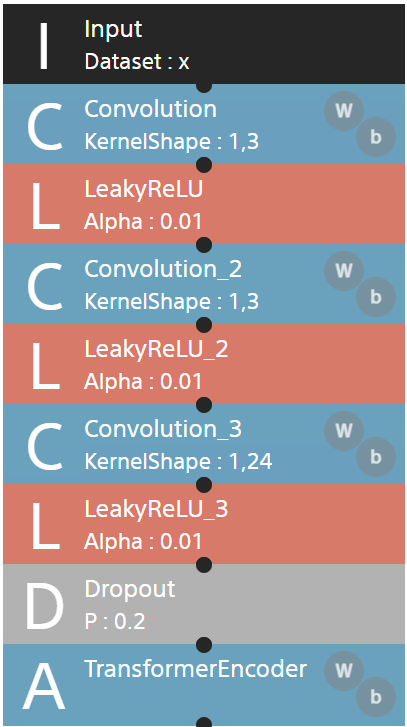
\includegraphics[width=0.5\linewidth]{./img/feature_extractor.png}
\end{center}
\caption{Feature Extractor CNN}
\end{figure}

\section{Results of t-SNE}
Since we needed to visualize the feature mapping when implementing DDLM, we implemented and ran t-SNE, which was also used in the DDLM paper.
Using t-SNE, we reduced the 64-dimensional features of the MNIST handwritten digit dataset to two dimensions and visualized them as shown in the figure below.

In the figure, you can see that each of the handwritten features from 0 to 9 is mapped as a cluster.

\begin{figure}[H]
\begin{center}
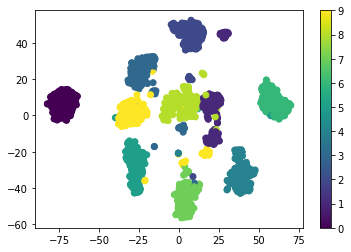
\includegraphics[width=0.8\linewidth]{./img/mnist_t-SNE.png}
\end{center}
\caption{Mapping of handwritten character features}
\end{figure}

\section{Next Plan}
\begin{itemize}
    \item Apply public MATLAB code \cite{matlab} to the dataset for preprocessing
    \item Extract features from the heartbeat signal in the dataset \cite{dataset} using CNN and visualize it using t-SNE
\end{itemize}

\begin{thebibliography}{99}
\bibitem{ddlm} Yan, Baiju, et al. ”Heart signatures: Open-set person identification based on cardiac radar signals.” Biomedical Signal Processing and Control 72 (2022): 103306.
\bibitem{matlab} \url{https://gitlab.com/sven_schellenberger/scidata_phase1}
\bibitem{dataset} \url{https://figshare.com/articles/dataset/A_dataset_of_clinically_recorded_radar_vital_signs_with_synchronised_reference_sensor_signals/12186516?file=22515782}
\end{thebibliography}
\end{document}